%include exam documentclass
\documentclass{exam} 
\usepackage{fullpage}
\usepackage{amsmath}
\usepackage{comment}
\usepackage{graphicx}

\begin{document}

%print header
\examheader{CISC 106}{UEF Example}{Developed: 2010}

%example of a block
\begin{block}{example topic}
  This is a block.
\end{block}

%example figure
\begin{figure}[placement h]
  \begin{center}
      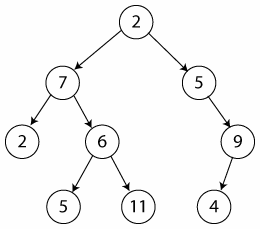
\includegraphics[scale=0.50]{binary_tree.png}
      \caption{Example Figure}
      \label{fig:example topic}
   \end{center}
\end{figure}

%example of a problem, require block:example topic
%and fig:example topic
\begin{problem}[require=example topic]{example topic}{15}
  #1: This is a problem that requires a figure 
  \ref{fig:example topic}
  \begin{answers}
    \answer[correct] correct answer 1
    \answer answer 2
    \answer[fixed] fixed answer 3
    \answer[correct,fixed] correct fixed answer 4
    \answer answer 5
    \answer[fixed,correct] fixed correct answer 6
  \end{answers}
\end{problem}

%example of a problem, require block:example topic
%and fig:example topic
\begin{problem}[require=example topic]{example topic}{15}
  #2: This is a problem that requires a figure
  \ref{fig:example topic}
  \begin{answers}
    \answer[correct] correct answer 1
    \answer answer 2
    \answer[fixed] fixed answer 3
    \answer[correct,fixed] correct fixed answer 4
    \answer answer 5
    \answer[fixed,correct] fixed correct answer 6
  \end{answers}
\end{problem}
%example of a problem, require block:example topic
%and fig:example topic
\begin{problem}{example topic}{15}
  #3: This is a problem that doesn't
  \ref{fig:example topic}
  \begin{answers}
    \answer[correct] correct answer 1
    \answer answer 2
    \answer[fixed] fixed answer 3
    \answer[correct,fixed] correct fixed answer 4
    \answer answer 5
    \answer[fixed,correct] fixed correct answer 6
  \end{answers}
\end{problem}



\end{document}







